\documentclass[border=0.2cm]{standalone}

%\renewcommand{\raggedsection}{\centering}
\usepackage{graphicx}
\usepackage{sectsty}
\usepackage{lipsum}
\usepackage{cases}
\usepackage{tikz}
\usetikzlibrary{shapes.geometric}
\usetikzlibrary{calc}
\usetikzlibrary{arrows}
\usetikzlibrary{decorations.pathreplacing}
\usetikzlibrary{arrows.meta}

\begin{document}
	\begin{tikzpicture}[state/.style={rectangle, draw, rotate=90, minimum width=80pt}]
		\pgfmathsetmacro{\cubex}{1.8}
		\pgfmathsetmacro{\cubey}{1.8}
		\pgfmathsetmacro{\cubez}{1.8}

		% NeuralSampler
		\node[inner sep=0pt] (input_ptc) at (-8,4) {\frame{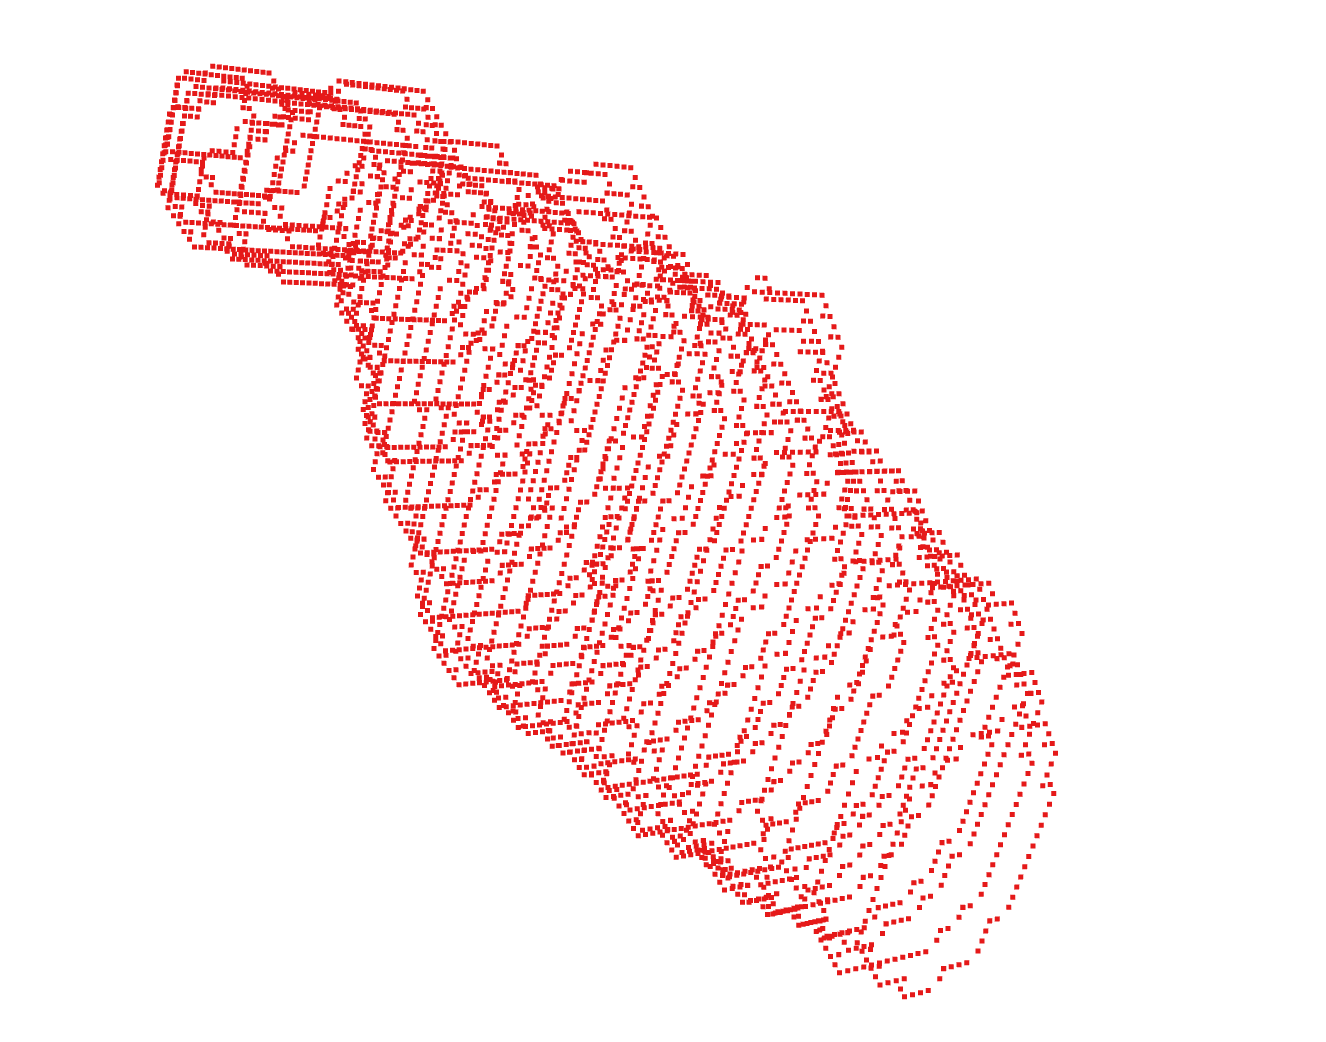
\includegraphics[width=.2\textwidth]{ptc.png}}};
		\node (input) at (-8,2.85) {\tiny input};
		\node (input_size) at (-8,5.15) {\tiny Px3};

		\node (pn) at (-5,4) {PointNet};
		\draw ($(pn.north west)+(-0.7, 1.05)$) rectangle ($(pn.north east)+(0.7,-1.55)$);
		\node[state] (grid) at (-3,4) {gridpooling};
		%\draw (-0.5,4.8,0) -- ++(-\cubex,0,0) -- ++(0,-\cubey,0) -- ++(\cubex,0,0) -- cycle;
		%\draw (-0.5,4.8,0) -- ++(0,0,-\cubez) -- ++(0,-\cubey,0) -- ++(0,0,\cubez) -- cycle;
		%\draw (-0.5,4.8,0) -- ++(-\cubex,0,0) -- ++(0,0,-\cubez) -- ++(\cubex,0,0) -- cycle;
		\node [trapezium, trapezium angle=60, minimum width=80pt, draw, rotate=-90] (resnet) at (-0.5,4){};
		\node (resnet_text) at (-0.5,4){\tiny ResNet};
		\node[rectangle, draw, minimum width=25pt] (l) at (0.75,4){\scriptsize L};
		\node [trapezium, trapezium angle=60, minimum width=80pt, draw, rotate=90] (resnet-1) at (2,4){};
		\node (resnet-1_text) at (2,4){\tiny ResNet$^-1$};

		\node (sampling) at (5.8,4) {\begin{tabular}{c}Sampling  \\ layer\end{tabular}};
		\draw ($(sampling.north west)+(-0.5, 0.8)$) rectangle ($(sampling.north east)+(0.5,-1.8)$);

		\node[inner sep=0pt] (output_ptc) at (10,4) {\frame{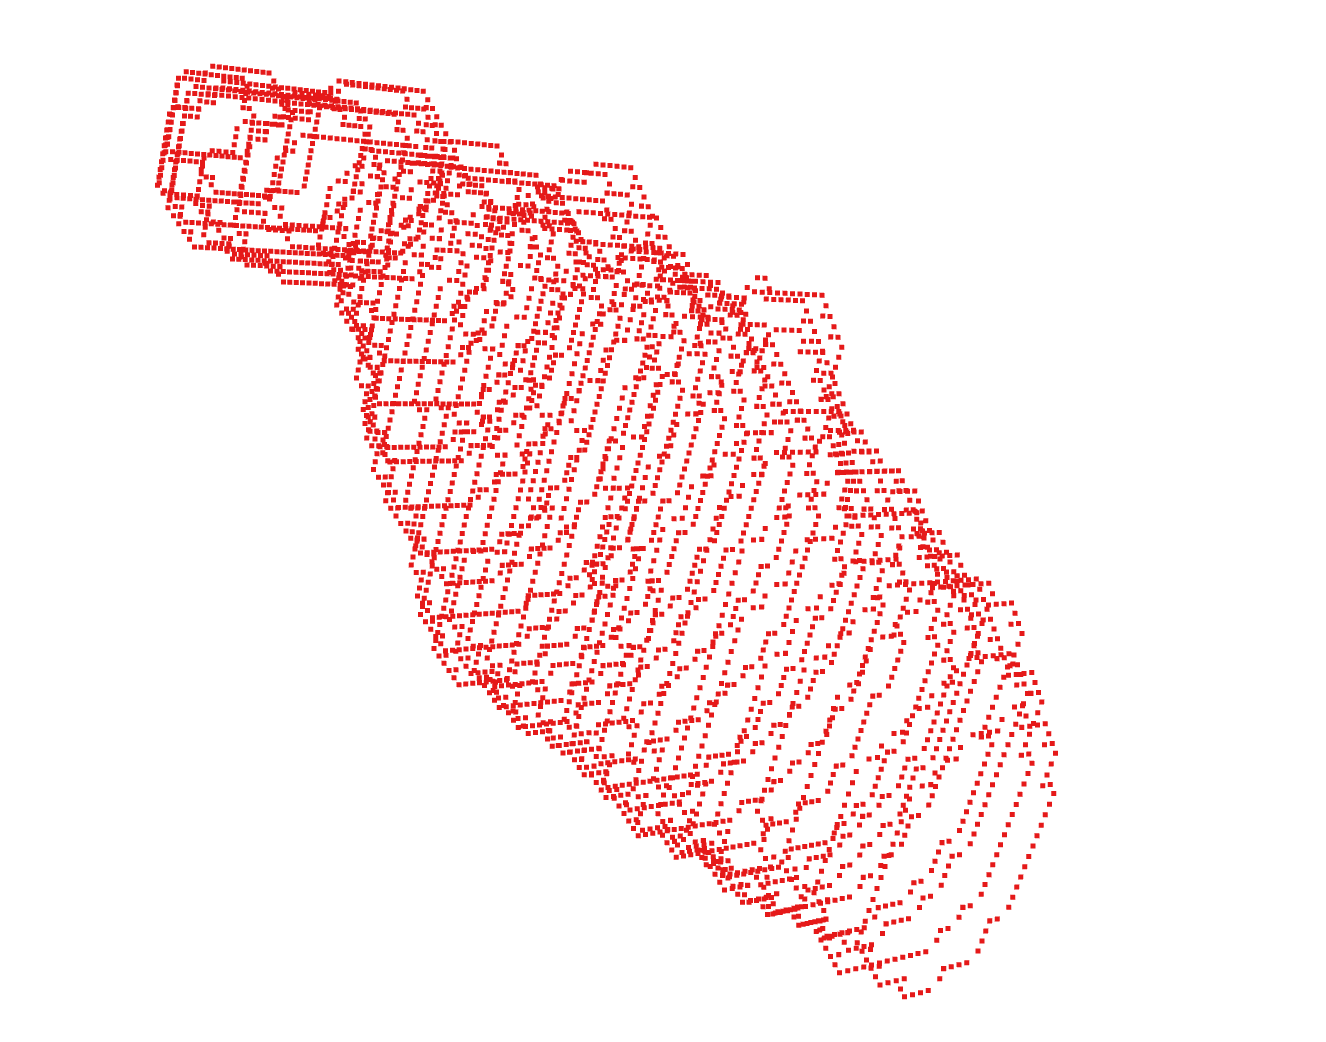
\includegraphics[width=.2\textwidth]{ptc.png}}};
		\node (input) at (10,2.85) {\tiny reconstruction};
		\node (input_size) at (10,5.15) {\tiny Qx3};
		
		%\path [line width=0.1pt] (pn) edge (grid);
		\path [->, -latex, line width=0.1pt] (input_ptc) edge ($(pn.west)+(-0.7,0)$);
		\path [->, -latex, line width=0.1pt] (grid) edge node [above] {\tiny FxNxNxN} (resnet); %$F\times N\times N\times N$
		\path [->, -latex, line width=0.1pt] (resnet-1) edge node [above] {\tiny 1xNxNxN}  node [below] {\tiny occupancy} ($(sampling.west)+(-0.5,0)$);
		\path [->, -latex, line width=0.1pt] ($(sampling.east)+(0.5,0)$) edge node [above] {\tiny 3xNxNxN} node [below] {\tiny offset} (output_ptc);

		\node (lossbce) at ($(sampling.west)+(-1.25,-2)$) {\scriptsize $\mathcal{L}_{BCE}$};
		\node (losschamfer) at (10,2) {\scriptsize $\mathcal{L}_{Chamfer}$};
		\path [line width=0.1pt] (3.5, 3.5) edge (lossbce);
		\path [line width=0.1pt] (10, 2.5) edge (losschamfer);
		
		
		%%%%%%%%%%%%%%%%%%%%%%%%%%%%%%%%%%%%%%%%%%%%%%%%%%%%%%%%%%%%%%%%%%%%
		% Pointnet
		\node[state] (n1) at (-4,0) {$n \times 3$};
		\node[rectangle,draw] (in_trans) at (-3,0) {};
		\node[state] (n2) at (-2,0) {$n \times 3$};
		\node[state] (n3) at (0,0) {$n \times 64$};
		\node[rectangle,draw] (feat_trans) at (1,0) {};
		\node[state] (n4) at (2,0) {$n \times 64$};
		\node[state] (n5) at (4,0) {$n \times 512$};
		\draw (4.4, 1.04) -- (4.4, -1.04) -- (5,0)-- cycle;
		\node (pool) at (5.2, 0.6) {\tiny \begin{tabular}{c}max \\ pooling \end{tabular}};
		\node[rectangle,draw, minimum width=80pt] (n6) at (7,0) {512};
		
		% description nodes
		\node (desc) at (7.1,-0.5) {\tiny latent representation};
		\node (desc2) at (7.75,-3.5) {PointNet};
		\node (desc3) at (-1,0.75) {\tiny \begin{tabular}{c}convolutional \\ layers \end{tabular}};
		\node (desc3) at (3,0.75) {\tiny \begin{tabular}{c}convolutional \\ layers \end{tabular}};
		
		
		%T-Net 1 
		\node[rectangle,draw, minimum height=15pt, rounded corners=1ex] (tnet) at (-2.5,-2) {\tiny T-Net};
		\node[rectangle,draw, rounded corners=1ex] (matr_m) at (-2,-3) {\tiny \begin{tabular}{c}matrix \\ mulitply \end{tabular}};
		\path [->, -latex, line width=0.1pt] (tnet) edge (matr_m);
		\path [->, -latex, line width=0.1pt] (-3.75, -3) edge (matr_m);
		\path [->, -latex, line width=0.1pt] (-3.5, -3) edge (tnet);
		\path [->, -latex, line width=0.1pt] (matr_m) edge (-0.8, -3);
		\draw [dashed, line width=0.1pt, rounded corners=1ex] ($(tnet.north west)+(-0.65, 0.1)$) rectangle ($(matr_m.north east)+(0.2,-0.75)$);
		\node (trans3x3) at (-1.7,-2.3) {\tiny \begin{tabular}{c}3x3 \\ transform \end{tabular}};

		%T-Net 2 
		\node[rectangle,draw, minimum height=15pt, rounded corners=1ex] (tnet2) at (1.5,-2) {\tiny T-Net};
		\node[rectangle,draw, rounded corners=1ex] (matr_m2) at (2,-3) {\tiny \begin{tabular}{c}matrix \\ mulitply \end{tabular}};
		\path [->, -latex, line width=0.1pt] (tnet2) edge (matr_m2);
		\path [->, -latex, line width=0.1pt] (0.25, -3) edge (matr_m2);
		\path [->, -latex, line width=0.1pt] (0.5, -3) edge (tnet2);
		\path [->, -latex, line width=0.1pt] (matr_m2) edge (3.2, -3);
		\draw [dashed, line width=0.1pt, rounded corners=1ex] ($(tnet2.north west)+(-0.65, 0.1)$) rectangle ($(matr_m2.north east)+(0.2,-0.75)$);
		\node (trans3x3) at (2.3,-2.3) {\tiny \begin{tabular}{c}64x64 \\ transform \end{tabular}};
		
		% Networkpaths
		\path [->, -latex, line width=0.1pt] (n1) edge (in_trans);
		\path [->, -latex, line width=0.1pt] (in_trans) edge(n2);
		\path [->, -latex, line width=0.1pt] (n2) edge node [above] {\tiny [64,64]} (n3);
		\path [->, -latex, line width=0.1pt] (n3) edge (feat_trans);
		\path [->, -latex, line width=0.1pt] (feat_trans) edge (n4);
		\path [->, -latex, line width=0.1pt] (n4) edge node [above] {\tiny [64,128,512]} (n5);

		\path [dashed, line width=0.1pt] (in_trans) edge (tnet);
		\path [dashed, line width=0.1pt] (feat_trans) edge (tnet2);
		
		\draw [dashed, line width=0.1pt, rounded corners=1ex] ($(n1.north west)+(-0.5, 3)$) rectangle ($(n6.north east)+(0.5,-4)$);

		%combine
		\path [dashed, line width=0.1pt] ($(pn.south)+(0,-1.05)$) edge ($(n1.north west)+(-0.5, 3)$);
		%\path [->, -latex, line width=0.1pt] (res1) edge node [below] {\tiny 3x3x1} (res2);
	\end{tikzpicture}
\end{document}
